\section{线程粗化与完整归约实现}
\label{l15:sec:coarse}

\subsection{增加每个线程承担的局部工作}

前面的未粗化实现让每个线程先处理两个输入，再进入块内归约。对很大的输入，线程块数量可能远多于硬件能同时驻留的块数，块会分批执行。每批数据都会再次经历归约树从高并行度逐渐收缩到低并行度的过程，并支付相应的块内通信代价。

线程粗化（thread coarsening）让同一个线程先顺序合并更多输入，再执行一次块内归约。设粗化因子为正整数 $C$，则每个线程负责 $2C$ 个输入，每个块处理 $2CB$ 个输入，段首改为 $s_b=2CBb$。每个线程在寄存器中形成
\begin{equation}
v_t=\sum_{j=0}^{2C-1}\widetilde x_{s_b+t+jB},
\qquad
\widetilde x_i=
\begin{cases}
x_i,&i<N,\\
0,&i\geq N.
\end{cases}
\label{l15:eq:coarse-local}
\end{equation}
这里 $\widetilde x_i$ 表示逻辑补零后的输入，无需真的分配填充数组。完成局部累加后，只需再对 $B$ 个 $v_t$ 使用前面任一种块内归约结构。

地址 $s_b+t+jB$ 使同一轮 $j$ 中相邻线程访问连续位置。以 $B=128$、$C=2$、$b=0$ 为例，线程 $5$ 读取下标 $5,133,261,389$，线程 $6$ 读取 $6,134,262,390$。每个线程沿自己的序列顺序累加，而各线程的同一轮访问仍组成连续地址区间。图\ref{l15:fig:coarse} 用较小的线程数展示这种结构。

\begin{figure}[htbp]
\centering
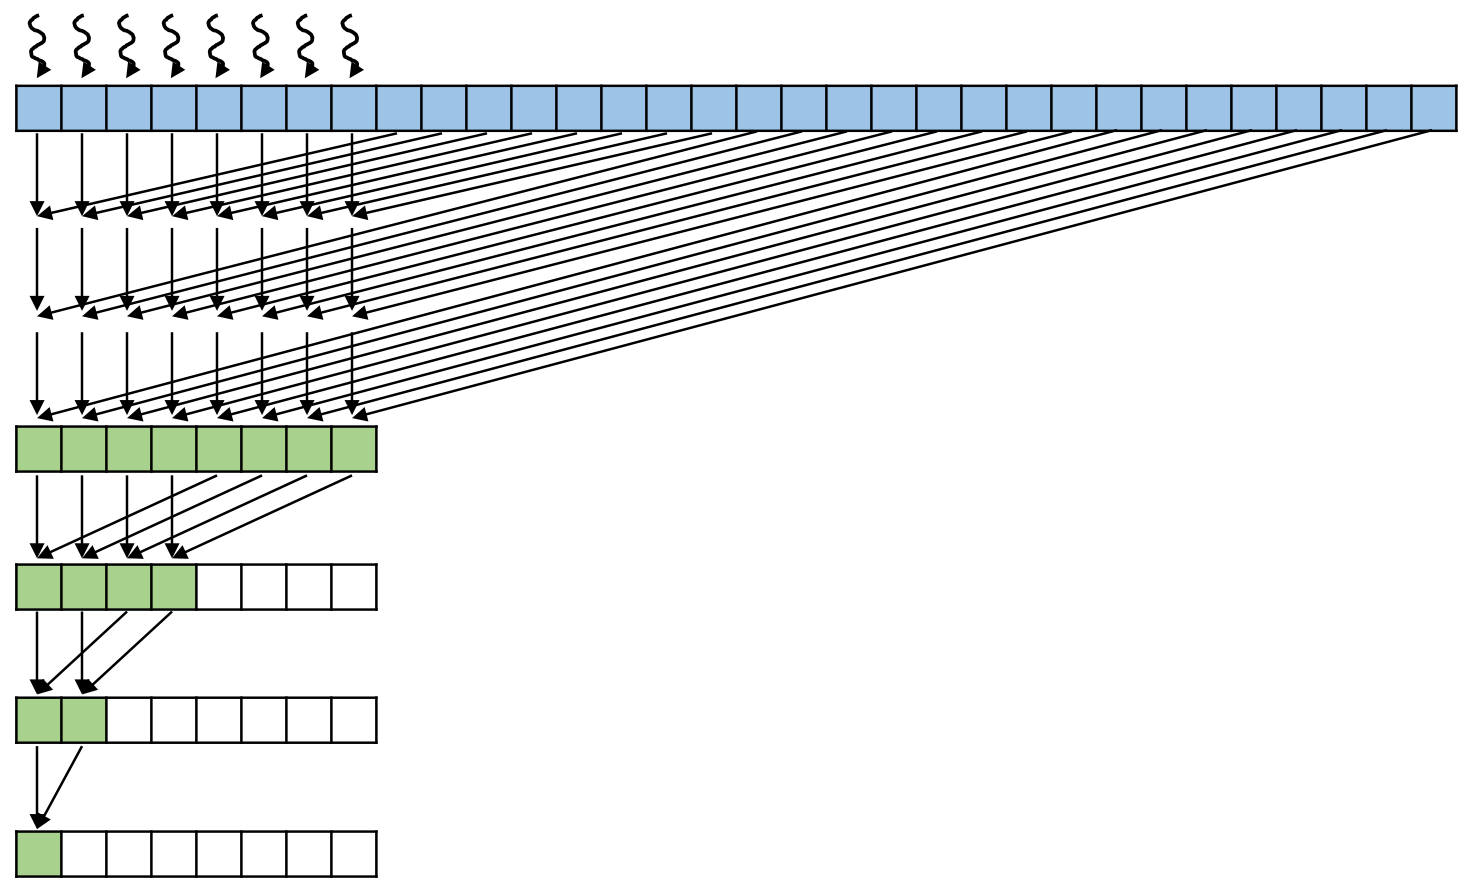
\includegraphics[width=0.82\linewidth]{thread-coarsening.png}
\caption{图示采用八个线程，每个线程先累加四个输入，再对八个局部部分和进行树形归约。上方的多轮读取保持跨线程的连续地址关系。}
\label{l15:fig:coarse}
\end{figure}

块数随之变为 $G_C=\lceil N/(2CB)\rceil$。与未粗化相比，局部顺序工作增多，而需要启动和归约的线程块减少，块间原子更新数或写出的块结果数也随之减少。这个取舍在原本块数充足、硬件不得不分批处理时尤其有意义。

\subsection{工作量、阶段数与同步次数的比较}

为分析粗化如何改变树尾的重复开销，令原始每块输入数为 $M_0=2B$，并取 $B$ 为二的幂。原始块内树深度为 $L_B=\log_2M_0=1+\log_2B$。以下先使用单位加法时间、忽略数据传输细节的理想模型，比较处理同样 $2CB$ 个输入时的局部阶段数。

若未粗化的 $C$ 个块必须由硬件依次执行，则需要约 $CL_B$ 个阶段。粗化后，每个线程先把 $2C$ 个值顺序合为一个值，沿该线程的依赖链需要 $2C-1$ 次加法；之后再运行深度为 $\log_2B$ 的块内树。因此，粗化后的跨度和必要工作量为
\begin{align}
D_C&=(2C-1)+\log_2B=2(C-1)+L_B,
\label{l15:eq:coarse-depth}\\
W_C&=B(2C-1)+(B-1)=2CB-1.
\label{l15:eq:coarse-work}
\end{align}
工作量仍恰好等于把 $2CB$ 个值合并成一个值所需的次数。未粗化的 $C$ 个块内部一共做 $C(2B-1)$ 次必要加法，若再把这 $C$ 个块和合成一个结果，还要做 $C-1$ 次，因此总数同样是 $2CB-1$。两种方案主要改变工作在线程内部、块内部和块之间的分配。

上述 $CL_B$ 只计原有数据段依次完成块级输出的阶段，得到的是 $C$ 个块和；粗化后的一个块直接输出覆盖同样数据的一个块和。实际总耗时还应考虑最后的块间合并。若原来的 $C$ 个块本就能同时执行，则它们局部归约的并行深度只有 $L_B$，粗化反而增加了线程内部的顺序依赖，因此粗化因子增大不保证获得更短的时间。

以 $B=128$、$C=4$ 为例，原始每块有 $M_0=256$ 个输入，$L_B=8$。四个块顺次执行的局部阶段数为 $4\times8=32$；粗化后，一个块处理 $1024$ 个输入，每线程合并八个值需要七次加法，再经过七层块内树，共 $7+7=14$ 个阶段。这与式\eqref{l15:eq:coarse-depth} 的 $2(4-1)+8=14$ 一致。$32/14\approx2.29$ 是这一理想模型中的阶段数比，并非实测加速比。

同步次数必须按实际块内实现分别计算。若采用每个树层末尾均保留块屏障的经典结构，$C$ 个原始块共有 $CL_B$ 次块屏障调用，粗化后只需对 $B$ 个局部值执行一次归约，连同共享值初始化后的屏障，共 $L_B$ 次。对于 $B=128,C=4$，计数从 $32$ 次降至 $8$ 次。若已经采用两阶段线程束归约，则每块原本只有一次块屏障，粗化把对应的 $C$ 次降为一次，即这里的 $4\to1$。

因此，选择 $C$ 时需要同时观察局部顺序依赖、块数和同步开销。较大的 $C$ 能减少重复的块内归约及块结果写出，但也会减少可调度的块数；输入规模较小时，剩余块数可能不足以利用所有计算资源。循环展开及更多同时保留的中间值还可能提高寄存器占用。实际参数应依据固定输入规模下的运行时间比较，并保持相同的计时范围和数值正确性标准。

式\eqref{l15:eq:coarse-depth} 使用的是理想二叉块内树。若采用固定 $32$ 通道的两阶段交换代码，补零通道及不再进入最终结果的通道仍会执行部分指令，实际指令路径不必恰好等于这个理想层数。阶段数模型解释了粗化的来源，最终性能仍由所用代码与硬件共同决定。

\subsection{完整核函数与块间合并}

下面把每线程局部累加、两阶段线程束归约和最终输出连接起来。实现采用 C++17，使用前面定义的 \mbox{\code{warp_sum}} 辅助函数；源文件包含 \mbox{\code{<cuda_runtime.h>}} 和 \mbox{\code{<cstddef>}}。模板参数 $B$ 表示每块线程数，$C$ 表示粗化因子，编译期布尔参数 \mbox{\code{AtomicOutput}} 选择直接原子累加总和，或写出每个块的部分和。

对一个完整块，初始化直接读取每个线程的第一个输入，后面的循环进行 $2C-1$ 次加法，与前面的局部跨度计数一致。尾块的读取分别检查边界，缺少输入的线程保留零或已有部分和，并继续参加完整的线程束归约。输入索引在乘法之前转换为 \mbox{\code{size_t}}，避免先用较窄整数计算大数组地址。

输出选择只在每块的第 $0$ 个线程执行。采用原子输出时，输出只需一个浮点数，在所有块开始累加前初始化一次为 $0$；采用部分和输出时，输出需要 $G_C$ 个浮点数，由各块分别覆盖自己的位置。两种模式均要求输出区间不与当前输入重叠。

\noindent\begin{minipage}{\linewidth}
\begin{lstlisting}[caption={带线程粗化的完整归约核函数},label={l15:lst:code4}]
template<int B, int C, bool AtomicOutput>
__global__ void reduce_coarsened(const float* input,
                                 size_t n, float* output) {
    static_assert(B >= 32 && B <= 1024 && B % 32 == 0,
                  "B must contain complete warps");
    static_assert(C >= 1, "C must be positive");
    constexpr int Q = B / 32;
    __shared__ float warp_totals[Q];
    unsigned int t = threadIdx.x;
    size_t i = size_t(2) * C * B * blockIdx.x + t;

    float value = (i < n) ? input[i] : 0.0f;
    for (size_t tile = 1; tile < size_t(2) * C; ++tile) {
        size_t j = i + tile * B;
        if (j < n) value += input[j];
    }

    value = warp_sum(value);
    if (t % 32 == 0) warp_totals[t / 32] = value;
    __syncthreads();

    if (t < 32) {
        value = (t < Q) ? warp_totals[t] : 0.0f;
        value = warp_sum(value);
        if (t == 0) {
            if constexpr (AtomicOutput) {
                atomicAdd(output, value);
            } else {
                output[blockIdx.x] = value;
            }
        }
    }
}
\end{lstlisting}
\end{minipage}

原子模式可以使用下面的主机端启动函数。输入和输出指针均指向已经分配好的设备内存，块数应在设备允许的网格范围内。初始化与核函数在同一执行流（stream）中提交，使清零先于所有块的累加执行。

\noindent\begin{minipage}{\linewidth}
\begin{lstlisting}[caption={在同一执行流中初始化输出并启动归约},label={l15:lst:code5}]
template<int B, int C>
cudaError_t launch_atomic_sum(const float* input,
                             size_t n, float* sum,
                             cudaStream_t stream = nullptr) {
    cudaError_t status =
        cudaMemsetAsync(sum, 0, sizeof(float), stream);
    if (status != cudaSuccess || n == 0) return status;

    constexpr size_t chunk = size_t(2) * B * C;
    size_t blocks = n / chunk + (n % chunk != 0);
    reduce_coarsened<B, C, true>
        <<<static_cast<unsigned int>(blocks), B, 0, stream>>>
        (input, n, sum);
    return cudaGetLastError();
}
\end{lstlisting}
\end{minipage}

以 $B=256,C=4$ 为例，每块处理 $2048$ 个输入。调用时将 \mbox{\code{launch_atomic_sum}} 的两个模板实参依次设为 $256$ 和 $4$。空输入只执行输出清零，不启动零个线程块的核函数。启动函数是异步提交：返回的状态用于检查提交和启动错误；主机要读取数值时，还需等待该执行流完成并检查执行错误，再把设备结果复制到主机。

采用多轮部分和归约时，把 \mbox{\code{AtomicOutput}} 设为 \mbox{\code{false}}。空输入直接把最终结果设为单位元 $0$，单元素输入可以直接返回或复制该值，均无需进入多轮过程。以下递推取 $N\geq2$，设当前输入长度为 $n_k$，每块容量为 $M=2BC$，则下一轮的输入长度为
\begin{equation}
n_{k+1}=\left\lceil\frac{n_k}{M}\right\rceil,
\qquad n_0=N.
\label{l15:eq:multipass}
\end{equation}
第一轮从原始输入写入临时数组，后续在两个互不重叠的临时数组之间交替读写，直到只剩一个部分和。每轮在同一执行流中依次提交，核函数边界为下一轮提供完整的块间阶段顺序。部分和输出模式会覆盖本轮的全部有效输出位置，因此这些输出槽位不需要像原子总和那样预先清零。

两种块间合并方法的主要差别是，原子模式用一次核函数完成所有块的局部计算，并竞争同一个最终地址；多轮模式把块间合并继续表示成较小的归约任务，需要额外的核函数启动和临时结果读写。输入规模、块数和设备特性共同决定其性能，比较时应包含所选方案完成一次归约实际需要的全部阶段。
